\documentclass[11pt]{article}

\usepackage[letterpaper,margin=1in]{geometry}
\usepackage{amsmath,amssymb,amsthm,mathtools}
\usepackage{booktabs,tabularx,array}
\usepackage{enumitem}
\usepackage{xcolor}
\usepackage{graphicx}
\usepackage{tikz}
\usetikzlibrary{arrows.meta,calc,positioning,fit,decorations.pathreplacing}
\usepackage{microtype}
\usepackage{fancyhdr}
\usepackage[colorlinks=true,linkcolor=blue!45!black,urlcolor=blue!45!black]{hyperref}

\definecolor{youngblue}{RGB}{29,94,145}
\definecolor{oldorange}{RGB}{172,83,32}
\definecolor{plannergreen}{RGB}{46,119,78}
\definecolor{softgray}{RGB}{242,244,247}
\definecolor{darkgray}{RGB}{70,74,80}

\setlength{\parindent}{0pt}
\setlength{\parskip}{0.55em}
\setlength{\emergencystretch}{3em}
\allowdisplaybreaks
\setlist[itemize]{leftmargin=1.35em,itemsep=0.18em,topsep=0.2em}
\setlist[enumerate]{leftmargin=1.55em,itemsep=0.18em,topsep=0.2em}

\newtheorem{proposition}{Proposition}
\newtheorem{lemma}{Lemma}
\newtheorem{corollary}{Corollary}
\newtheorem{definition}{Definition}
\newtheorem{assumption}{Assumption}
\newtheorem{remark}{Remark}

\newcommand{\dd}{\mathrm d}
\newcommand{\1}{\mathbf 1}
\newcommand{\E}{\mathbb E}
\newcommand{\CV}{\operatorname{CV}}
\newcommand{\MRS}{\operatorname{MRS}}
\newcommand{\Nu}{\mathcal N}
\newcommand{\cY}{c^{Y}}
\newcommand{\hY}{h^{Y}}
\newcommand{\cO}{c^{O}}
\newcommand{\hO}{h^{O}}
\newcommand{\ellbar}{\bar\ell}
\newcommand{\zF}{\zeta^{O,F}}
\newcolumntype{L}[1]{>{\raggedright\arraybackslash}p{#1}}
\newcolumntype{Y}{>{\raggedright\arraybackslash}X}

\pagestyle{fancy}
\setlength{\headheight}{14pt}
\fancyhf{}
\fancyhead[L]{Housing access, retention, and efficiency}
\fancyhead[R]{Proof audit}
\fancyfoot[C]{\thepage}
\renewcommand{\headrulewidth}{0.35pt}

\title{\textbf{Housing Access, Old-Owner Retention, and Efficiency}\\[0.35em]
\large A complete accounting and proof audit of the simplified model}
\author{Technical note for the paper draft}
\date{July 2026}

\begin{document}
\maketitle

\begin{abstract}
This note reconstructs the simplified two-period housing model from its
primitive budgets and derives the strongest efficiency statements that the
environment can support. The accounting dispute has a precise resolution.
For a constrained young owner, $r+\zeta^{O,F}$ is her private lifetime
willingness to pay for a marginal unit after accounting for the future tax.
It is not the fiscal-inclusive social value. If the marginal unit generates a
future capital-gains tax and the revenue is rebated inside the planner's
boundary, its present value $q\bar\ell$ must be added back. Against an old
incumbent whose marginal value is $r-\bar\ell$, the correct local
consumption-equivalent surplus is therefore
\(\zeta^{O,F}+q\bar\ell+\bar\ell\). The coefficient $q\bar\ell$ is exact
along an explicitly constructed path that holds the recipient's future
retention fixed and releases the added carried unit; interiority alone does not
imply that path. With no gains tax, the financing wedge alone produces a
first-best Pareto improvement when the planner can bypass the down-payment
constraint. A genuinely constrained result is also available after a minimal
implementation closure: aggregate old retention raises the equilibrium house
price, and the higher price tightens young buyers' down-payment constraints.
The relevant price response is the response of a \emph{joint compensated
equilibrium}, because the transfers used to hold households harmless affect
their demands. A compensated tax on current old retention then yields the
surplus $-P_\tau^c\mathcal K>0$ while the same underwriting rule remains in
force. This theorem is a one-date, fixed-cross-section result, not a comparison
of stationary dynamic equilibria. The full dynamic planner is not closed by
the note as written; the missing fiscal, asset, maintenance, bequest,
outside-option, and population-welfare accounts are stated explicitly below.
\end{abstract}

\vspace{0.35em}
\begin{center}
\begin{minipage}{0.94\textwidth}
\small
\textbf{Bottom line.} The purchase-price term is not being counted twice.
The disputed $q\bar\ell$ is the date-$t$ value of a date-$t+1$ fiscal receipt.
The original local expression can be correct, but only after distinguishing a
static marginal rate of substitution, a private lifetime willingness to pay,
and a fiscal-inclusive social value. The local result is a first-best result.
The constrained result requires a compensated general-equilibrium price
response and is not implied by a positive private multiplier alone. The
current note must add the settlement and passive-sector closure before that
result can be stated as a theorem.
\end{minipage}
\end{center}

\clearpage
\setcounter{tocdepth}{1}
\begingroup
\setlength{\parskip}{0pt}
\tableofcontents
\endgroup
\clearpage

% ================================================================
\section{Verdict}
% ================================================================

The simplified model supports two informative but distinct efficiency
results. It does not support an unconditional full welfare theorem without a
small set of additional accounting closures.

\begin{center}
\renewcommand{\arraystretch}{1.18}
\begin{tabularx}{\textwidth}{@{}L{0.22\textwidth}Y L{0.18\textwidth}@{}}
\toprule
Claim & Correct statement & Status \\
\midrule
Local first-best reallocation
& If a planner can place a marginal unit with a financially constrained young
owner and take it from an old owner at an interior release margin, the
consumption-equivalent surplus is
$\zeta_i^{O,F}+q\ellbar+\ellbar$, less real implementation costs.
& Valid under explicit margin and fiscal assumptions. \\
Finance alone
& At $\ellbar=0$, the same surplus is $\zeta_i^{O,F}>0$.
& Valid; the tax is not necessary. \\
Constrained inefficiency
& In a fixed-cross-section implementation economy, if a fully compensated
reduction in old retention lowers $P$ and the only active price-dependent
wedges are young down-payment constraints, the surplus is
$-P_\tau^c\mathcal K>0$.
& Valid after an explicit compensated-equilibrium and consolidated-account
closure; not proved by the current household equations alone. \\
Binding constraint alone
& A positive multiplier does not by itself establish constrained
inefficiency.
& False without an endogenous price or another social wedge. \\
Full dynamic efficiency
& A full theorem needs resource, fiscal, passive-sector, housing-supply,
bequest, outside-option, and population-welfare closures.
& Not established by the current note. \\
Discrete tenure
& Renter-to-owner and owner-to-renter changes require finite branch-value or
expenditure comparisons.
& No general marginal theorem. \\
\bottomrule
\end{tabularx}
\end{center}

The economically ambitious statement is the constrained one. It formalizes
the proposed mechanism: an individual old owner internalizes the value she
forgoes by retaining her house, but not the effect of aggregate retention on
the market price and hence on other households' required cash down payments.
That price effect is merely pecuniary when markets are complete. It becomes a
first-order social effect when $P$ appears in a binding collateral constraint.

% ================================================================
\section{Exact reconstruction of the simplified model}
\label{sec:reconstruction}
% ================================================================

This section takes the note literally. Interpretive repairs are separated from
the equations actually written.

\subsection{Agents, timing, and ownership}

At date $t$, a potential young household has type $i=(y_i,b_i)$, where $y_i$
is date-$t$ income and $b_i$ is liquid wealth at entry. After deciding whether
to enter the modeled market, an entrant chooses tenure $m_i\in\{R,O\}$,
current consumption $c_i$, occupied housing $h_i$, completed fertility $n_i$,
and expenditure $b_i'$ on a one-period bond. A young owner carries the chosen
house into date $t+1$; a young renter carries no house. At $t+1$, an old owner
chooses consumption $c_j^2$, retained housing $h_j^2$, and a terminal estate
$e_j$. An old renter chooses the same flow objects but has no carried house and
no capital-gains tax exposure.

The timing relevant for the proof is:
\begin{enumerate}
\item Young type and entry shocks are realized.
\item The young choose entry, tenure, $c_i,h_i,n_i,b_i'$ at prices $(P,r,q)$.
\item Current old incumbents choose how much of carried housing to retain;
      released units are sold during life and trigger the gains tax.
\item Current old households exit. Young owners carry $H_{i,t+1}^0=h_{i,t}$
      into old age; bond expenditure $b_i'$ pays $b_i'/q$ date-$t+1$ goods.
\item A marginal unit not retained by its old owner returns to the traded stock.
\end{enumerate}

\textit{Retention} is therefore a quantity, not a tenure label:
\[
\text{retained housing}=h_j^2,
\qquad
\text{released housing}=H_j^0-h_j^2.
\]
The old owner is permitted to downsize continuously because housing is
divisible. The model does not contain a genuine discrete old owner-to-renter
choice. With logarithmic old housing utility, $h_j^2=0$ is outside the domain,
so the old owner never fully exits ownership in the literal formulation.

\subsection{Preferences}

Young flow utility is
\begin{equation}
u_i^Y(c_i,h_i,n_i)
=\log(c_i-\chi n_i)+\alpha\log(h_i-\kappa n_i)
+\vartheta\log n_i,
\label{eq:young_utility}
\end{equation}
with domain $c_i>\chi n_i$, $h_i>\kappa n_i$, and $n_i>0$. Old utility is
\begin{equation}
u_j^O(c_j^2,h_j^2,e_j)
=\log c_j^2+\gamma\log h_j^2+\omega_B\log e_j.
\label{eq:old_utility}
\end{equation}
The warm-glow estate is not assigned to a modeled descendant in the simplified
note, and entry wealth is exogenous. That omission matters for a full
intergenerational planner, but not for the local housing proof.

\subsection{Prices and units}

There is a fixed, divisible stock $\bar H$. The asset price is $P$ and the
one-period housing user cost is $r$. The bond price is $q$, so one unit of
date-$t+1$ goods costs $q$ date-$t$ goods. No arbitrage imposes
\begin{equation}
r=\rho P,
\qquad
\rho=q^{-1}-1+\delta+\tau^p.
\label{eq:user_cost}
\end{equation}
The depreciation term is a real resource cost; interest and the foregone
return are intertemporal opportunity costs; property-tax payments are fiscal
transfers if rebated. For a local reallocation of a fixed total stock, the
common maintenance requirement is unchanged and cancels. It must reappear in
any planner problem that changes the stock.

Inflation at rate $\varpi$ creates a nominal taxable gain despite a constant
real asset price. A unit sold by an old owner generates the date-$t+1$ real tax
\begin{equation}
\ellbar=\tau^g\frac{P\varpi}{1+\varpi}.
\label{eq:gains_tax}
\end{equation}
For a current old seller, $\ellbar$ is current goods per unit. For a current
young buyer, the same numerical payment occurs next period and its date-$t$
value is $q\ellbar$.

\begin{center}
\renewcommand{\arraystretch}{1.15}
\begin{tabularx}{\textwidth}{@{}L{0.12\textwidth}L{0.39\textwidth}Y@{}}
\toprule
Object & Economic meaning & Units at date $t$ \\
\midrule
$P$ & Asset price of one housing unit & date-$t$ goods per housing unit \\
$r$ & One-period rent/user cost & date-$t$ goods per housing unit \\
$q$ & Bond price & date-$t$ goods per date-$t+1$ good \\
$b_i'$ & Expenditure on the bond & date-$t$ goods \\
$b_i'/q$ & Bond payoff & date-$t+1$ goods \\
$\ellbar$ & Tax paid when the unit is sold next period & date-$t+1$ goods per unit \\
$q\ellbar$ & Present value of that tax & date-$t$ goods per unit \\
$\lambda_i$ & Young budget multiplier & utility per date-$t$ good \\
$\mu_i$ & Down-payment multiplier & utility per date-$t$ good of slack \\
$\theta_i$ & Young size-cap multiplier & utility per housing unit of slack \\
$\xi_i$ & Bond lower-bound multiplier & utility per date-$t$ good of slack \\
$\eta_j$ & Old budget multiplier & old utility per date-$t+1$ good \\
$\zeta_i^{O,F}$ & Financing wedge & date-$t$ goods per housing unit \\
$\zeta_i^{O,S}$ & Owner-size wedge & date-$t$ goods per housing unit \\
\bottomrule
\end{tabularx}
\end{center}

The units already rule out one alleged error: $q\ellbar$ cannot be the purchase
price. The purchase price is $P$. The term $q\ellbar$ is a discounted future
tax flow.

\subsection{Young household problem}

Conditional on tenure $m$, the young household solves
\begin{align}
W_i^m=\max_{c_i,h_i,n_i,b_i'}\quad
&u_i^Y(c_i,h_i,n_i)
+\beta\left[\1\{m=R\}V^R(b_{j'})
+\1\{m=O\}V^O(b_{j'},h_i)\right] \\
\text{subject to}\quad
&c_i+r h_i+b_i'=y_i+b_i, \label{eq:young_budget}\\
&h_i\le \bar h^m,\qquad b_i'\ge0, \label{eq:young_bounds}\\
&\1\{m=O\}(1-\phi)Ph_i\le b_i. \label{eq:dp}
\end{align}
For owners, the generated old state is
\begin{equation}
b_{j'}=\frac{b_i'}q-rh_i,
\qquad H_{j'}^0=h_i;
\label{eq:owner_transition}
\end{equation}
for renters, $b_{j'}=b_i'/q$ and there is no carried house.

The common constraint $b_i'\ge0$ is imposed on \emph{both} tenure branches in
the written program. Thus the literal model does not merely say that renters
cannot borrow; owners cannot choose a negative bond position either. If that
restriction was intended to be tenure-specific, an indicator must be added to
\eqref{eq:young_bounds}.

Tenure is chosen by the finite comparison
\begin{equation}
W_i^Y=\max\{W_i^R,W_i^O\}.
\label{eq:tenure_choice}
\end{equation}
Equivalently, the two branch-specific housing caps are
\begin{equation}
H_i^O=\min\left\{\bar h^O,
\frac{b_i}{(1-\phi)P}\right\}
=\min\left\{\bar h^O,
\frac{b_i\rho}{(1-\phi)r}\right\},
\qquad H_i^R=\bar h^R.
\label{eq:effective_caps}
\end{equation}
With the note's logit entry shock, the probability of entering the modeled
market is
\begin{equation}
\pi_i^E=
\frac{\exp(W_i^Y/\kappa_E)}
{\exp(W_i^Y/\kappa_E)+\exp(\bar W^E/\kappa_E)}.
\label{eq:entry_probability}
\end{equation}
Hence any policy experiment that does not explicitly hold entry and tenure
branches fixed generally changes both the measure and the composition of
housing demand. This is why the constrained theorem below is stated for a
predetermined cross-section rather than by differentiating a stationary
entry equilibrium.

The down-payment rule uses $\phi$ as the financed share, so the required cash
share is $1-\phi$. In the written model, the inequality is an access test:
$P h_i$ does not appear as a goods use in \eqref{eq:young_budget}. This is
mathematically coherent as a reduced-form cap, but the phrase ``posts the down
payment out of liquid wealth'' is stronger than the ledger. The same $b_i$ is
both the right side of the access test and fully available in the flow budget.
A literal mortgage balance sheet would need separate equity and debt accounts;
Section~\ref{sec:missing} gives the minimal extension.

The term $-rh_i$ in \eqref{eq:owner_transition} is not an additional resource
cost by itself. It is the negative financial leg paired with the carried claim
$rH_{j'}^0$ in the old budget. With no gains tax, the two cancel exactly. The
model is therefore a flow-equivalent ownership ledger, not a literal record of
purchase principal $Ph_i$ and mortgage debt.

\subsection{Old household problems}

An old incumbent with state $(b_j,H_j^0)$ solves
\begin{align}
V^O(b_j,H_j^0)=\max_{c_j^2,h_j^2,e_j}\quad
&u_j^O(c_j^2,h_j^2,e_j) \\
\text{subject to}\quad
&c_j^2+e_j+r h_j^2
=b_j+rH_j^0-\ellbar(H_j^0-h_j^2),
\qquad 0\le h_j^2\le H_j^0.
\label{eq:old_owner_budget}
\end{align}
Equivalently,
\begin{equation}
c_j^2+e_j=(b_j)+(r-\ellbar)(H_j^0-h_j^2).
\label{eq:old_release_budget}
\end{equation}
Releasing one unit raises the old owner's spendable resources by
$r-\ellbar$: the gross sale value is $r$, the government receives $\ellbar$,
and the seller keeps the remainder. The maintained interior case requires
$0\le\ellbar<r$, $b_j+(r-\ellbar)H_j^0>0$, and
$0<h_j^2<H_j^0$.

Substituting the generated young-owner state \eqref{eq:owner_transition} into
\eqref{eq:old_owner_budget} gives
\begin{equation}
c_{j'}^2+e_{j'}+(r-\ellbar)h_{j'}^2
=\frac{b_i'}q-\ellbar h_i.
\label{eq:generated_old_budget}
\end{equation}
This identity is the cleanest check on the timing. Without the gains tax, old
consumption, bequests, and old housing services are financed by $b_i'/q$; the
purchase principal has netted out. With the tax, only units released during
life are taxed, but at an interior retention solution the envelope value of an
additional carried unit is its net sale value.

An old renter solves the same utility problem subject to
\begin{equation}
c_j^2+e_j+r h_j^2=b_j,
\qquad 0<h_j^2\le\bar h^R.
\label{eq:old_renter_budget}
\end{equation}

\subsection{Market clearing and passive sectors}

At a stationary cross-section, occupied housing satisfies
\begin{equation}
\bar M\int \pi_i^E h_i\,\dd G_Y(i)
+\int h_j^2\,\dd F_O(j)
+\int h_j^2\,\dd F_R(j)=\bar H.
\label{eq:housing_clearing}
\end{equation}
The note invokes passive landlords, a passive bond sector, lenders, and a
government, but does not write their budgets. For household optimality this is
innocuous. For welfare it is not: rents, house payments, mortgage principal,
interest receipts, and taxes are transfers only after the counterparties and
rebates are placed inside the social boundary.

% ================================================================
\section{Independent derivation of every marginal value}
\label{sec:derivation}
% ================================================================

\subsection{Old retention and envelope conditions}

Let $\eta_j$ be the multiplier on the old-owner budget. At an interior
retention choice, the first-order and envelope conditions are
\begin{equation}
\frac{u_{h,j}^O}{u_{c,j}^O}=r-\ellbar,
\qquad
V_b^O=\eta_j=u_{c,j}^O,
\qquad
V_H^O=(r-\ellbar)V_b^O.
\label{eq:old_envelopes}
\end{equation}
The first equality defines the retention margin. The old owner retains space
until its utility value equals the net amount she could obtain by releasing
it. With $\ellbar=0$, the old marginal value is exactly $r$.

At the upper corner $h_j^2=H_j^0$, equality is replaced by
$u_h^O/u_c^O\ge r-\ellbar$; the household would like to retain still more but
cannot. Such an owner is not automatically a valid donor for the local proof.
The interior assumption is substantive, not cosmetic.

\subsection{Young first-order conditions}

For a young owner, attach multipliers $\lambda_i$ to
\eqref{eq:young_budget}, $\mu_i$ to the slack form
$b_i-(1-\phi)Ph_i\ge0$, $\theta_i$ to $\bar h^O-h_i\ge0$, and $\xi_i$ to
$b_i'\ge0$. The saving and housing conditions are
\begin{align}
\lambda_i&=\frac{\beta}{q}V_b^O+\xi_i,
\label{eq:euler_general}\\
u_{h,i}^Y+\beta(V_H^O-rV_b^O)
&=\lambda_i r+\mu_i(1-\phi)P+\theta_i.
\label{eq:young_h_foc}
\end{align}
Define the date-$t$ value, in the young household's marginal utility units, of
one date-$t+1$ good:
\begin{equation}
d_i\equiv\frac{\beta V_b^O}{\lambda_i}
=q\left(1-\frac{\xi_i}{\lambda_i}\right)\le q.
\label{eq:di}
\end{equation}
For an interior saver, $\xi_i=0$ and $d_i=q$. Define the two goods-equivalent
access wedges
\begin{equation}
\zeta_i^{O,F}\equiv
\frac{\mu_i}{\lambda_i}(1-\phi)P,
\qquad
\zeta_i^{O,S}\equiv\frac{\theta_i}{\lambda_i}.
\label{eq:zetas}
\end{equation}
Both have units of current consumption per housing unit. Using
\eqref{eq:old_envelopes} in \eqref{eq:young_h_foc} yields the exact identity
\begin{equation}
\boxed{
\frac{u_{h,i}^Y}{u_{c,i}^Y}
=r+d_i\ellbar+\zeta_i^{O,F}+\zeta_i^{O,S}.}
\label{eq:young_static_mrs}
\end{equation}
For an interior saver with a slack owner size limit, this becomes
\begin{equation}
\frac{u_{h,i}^Y}{u_{c,i}^Y}
=r+q\ellbar+\zeta_i^{O,F}.
\label{eq:young_static_mrs_interior}
\end{equation}
This is the young household's \emph{current static MRS}. It includes the
current-goods value of the future tax because current housing utility must be
high enough to compensate for that future liability.

\subsection{The saving rule}

The log old-age problem provides a useful independent check. At an interior
old-owner solution, total net old resources are
\begin{equation}
S_i=\frac{b_i'}q-\ellbar h_i,
\end{equation}
which must be strictly positive.
and the old household allocates them with expenditure shares
\begin{equation}
c_{j'}^2=\frac{S_i}{1+\gamma+\omega_B},\qquad
(r-\ellbar)h_{j'}^2=\frac{\gamma S_i}{1+\gamma+\omega_B},\qquad
e_{j'}=\frac{\omega_B S_i}{1+\gamma+\omega_B}.
\label{eq:old_shares}
\end{equation}
Combining $V_b^O=1/c_{j'}^2$ with the interior Euler equation gives
\begin{equation}
\boxed{
b_i'=\beta(1+\gamma+\omega_B)(c_i-\chi n_i)
+q\ellbar h_i.}
\label{eq:saving_rule_verified}
\end{equation}
The last term is exactly the present cost of the marginal future tax. This
derivation independently verifies the coefficient $q$.

\subsection{Three objects that must not be conflated}

The source of the accounting dispute is now visible. For a young owner with a
slack owner size limit, define:
\begin{align}
m_i^{\mathrm{static}}
&\equiv\frac{u_{h,i}^Y}{u_{c,i}^Y}
=r+d_i\ellbar+\zeta_i^{O,F},
\label{eq:mstatic}\\
m_i^{\mathrm{private}}
&\equiv
\frac{u_{h,i}^Y+\beta(V_H^O-rV_b^O)}{u_{c,i}^Y}
=r+\zeta_i^{O,F},
\label{eq:mprivate}\\
m_i^{\mathrm{social}}
&\equiv m_i^{\mathrm{private}}+q\ellbar
=r+\zeta_i^{O,F}+q\ellbar.
\label{eq:msocial}
\end{align}
The second line is the household's private lifetime willingness to pay when
the extra unit changes both current housing and the generated old state. The
future tax reduces private continuation value, so it disappears from this
net object. The third line restores the present value of the government's
future receipt. It is the relevant fiscal-inclusive value when the government
can trade at $q$ and rebates revenue inside the planner's boundary.

For an interior old incumbent,
\begin{equation}
m_j^O=\frac{u_{h,j}^O}{u_{c,j}^O}=r-\ellbar.
\label{eq:mold}
\end{equation}
Therefore
\begin{equation}
\boxed{
m_i^{\mathrm{social}}-m_j^O
=\zeta_i^{O,F}+q\ellbar+\ellbar.}
\label{eq:correct_gap}
\end{equation}
The tentative correction $r+\zeta_i^{O,F}$ was a correct calculation of
$m_i^{\mathrm{private}}$. Calling it the social value omitted a fiscal asset.
Conversely, calling $r+q\ellbar+\zeta_i^{O,F}$ the young household's private
lifetime value would also be wrong. Equation \eqref{eq:correct_gap} is correct
only because the objects are named and consolidated consistently.

% ================================================================
\section{Correct local first-best proposition}
\label{sec:firstbest}
% ================================================================

\begin{assumption}[Local reallocation environment]
\label{ass:local}
At the competitive allocation: (i) housing is divisible and a marginal unit
can be reassigned without construction, conversion, matching, moving, or
underwriting costs; (ii) young owner $i$ has a slack physical owner-size limit,
a binding down-payment constraint with $\zeta_i^{O,F}>0$, and positive
effective consumption $c_i-\chi n_i>0$; (iii) current old owner $j$ has
$0<h_j^2<H_j^0$; (iv) the old retention problem generated by young owner $i$
has $0<h_{i,t+1}^2<H_{i,t+1}^0$; (v) prices, entry, tenure, fertility, and
saving are held fixed in the local variation; (vi) at date $t+1$ the planner
holds recipient $i$'s retained housing at its baseline value, releases the
additional carried unit, and adjusts $c_{i,t+1}^2$ and $e_{i,t+1}$ along their
conditional expenditure-minimizing shares; and (vii) the planner can implement
the transfer and use date-contingent lump-sum settlements, while current and
future tax receipts are rebated inside the social boundary and can be carried
across dates at price $q$. Passive ownership is adjusted so that the released
unit returns to the date-$t+1$ traded stock and physical housing clears.
\end{assumption}

\begin{proposition}[Correct local housing-allocation result]
\label{prop:local}
Under Assumption~\ref{ass:local}, the competitive allocation is locally Pareto
inefficient relative to a planner that does not face the private down-payment
constraint. Reassigning a marginal unit from old incumbent $j$ to young owner
$i$ generates the date-$t$ consumption-equivalent surplus
\begin{equation}
\boxed{
\mathcal S_{ij}'(0)
=\zeta_i^{O,F}+q\ellbar+\ellbar>0.}
\label{eq:local_surplus}
\end{equation}
If the reallocation has marginal real cost $k_{ij}\ge0$, the result holds if
$\zeta_i^{O,F}+q\ellbar+\ellbar>k_{ij}$.
\end{proposition}

\begin{proof}
Consider a transfer of $\varepsilon>0$ units with a flow-equivalent settlement
of $r\varepsilon$. This is the payment appearing in the reduced-form ledger;
it is not the literal asset purchase price $P\varepsilon$.
The old incumbent releases $\varepsilon$. Her spendable resources rise by
$(r-\ellbar)\varepsilon$, while her housing falls by $\varepsilon$. Using
\eqref{eq:old_envelopes}, her first-order utility change is
\[
u_{c,j}^O\big[(r-\ellbar)-u_{h,j}^O/u_{c,j}^O\big]\varepsilon=0.
\]
The gross payment $r\varepsilon$ is a transfer: the old household receives
$(r-\ellbar)\varepsilon$ and the government receives
$\ellbar\varepsilon$.

The young owner receives the unit and pays $r\varepsilon$, while $n_i$ and
$b_i'$ remain fixed. Her old state changes according to
\eqref{eq:owner_transition}. Her lifetime utility change, before an additional
lump-sum settlement, is
\begin{align*}
\big[u_{h,i}^Y+\beta(V_H^O-rV_b^O)-\lambda_i r\big]\varepsilon
&=\big[\mu_i(1-\phi)P+\theta_i\big]\varepsilon\\
&=\lambda_i\zeta_i^{O,F}\varepsilon,
\end{align*}
where the last equality uses the slack owner-size limit. The planner can
therefore levy a settlement charge
$\zeta_i^{O,F}\varepsilon+o(\varepsilon)$ after placing the unit, leaving the
young household at her original lifetime utility. The timing of this charge
is irrelevant for the first-best planner; it is not being used to satisfy the
private down-payment test.

It remains to construct, rather than assume, the future fiscal leg. At date
$t+1$, hold the recipient's retained housing $h_{i,t+1}^2$ at its baseline
value and release the added carried unit. Relative to the baseline old budget,
the extra carried unit and the $-r\varepsilon$ change in financial wealth
cancel at the gross user cost, while the additional sale reduces private net
resources by exactly $\ellbar\varepsilon$. Reduce $c_{i,t+1}^2$ and
$e_{i,t+1}$ by that total amount in their conditional expenditure-minimizing
shares. This produces exactly the continuation-utility derivative
$-V_b^O\ellbar\varepsilon$ already contained in
$V_H^O-rV_b^O=-\ellbar V_b^O$. Because the baseline retention choice is
interior, fixing it at its optimum rather than reoptimizing changes private
utility only at second order. The planner receives exactly
$\ellbar\varepsilon$ next period, worth $q\ellbar\varepsilon$ at date $t$,
and places the released physical unit in the passive/traded stock.

After both households have been held indifferent, the planner therefore has
\[
\big(\zeta_i^{O,F}+\ellbar+q\ellbar\big)\varepsilon
+o(\varepsilon)
\]
date-$t$ goods left over. By continuity, this residual is positive for all
sufficiently small $\varepsilon$. Giving the residual to either household (or
to any household with positive marginal utility of consumption) makes one
strictly better off and leaves all others weakly better off. This is a Pareto
improvement. A real implementation cost subtracts
$k_{ij}\varepsilon+o(\varepsilon)$ from the residual.
\end{proof}

The proof also explains why the old tax is counted once, not twice. The
flow-equivalent settlement is $r$. Of that amount, $r-\ellbar$ is exactly the
old owner's required net compensation and $\ellbar$ is available in the
government account. The future $q\ellbar$ is a separate tax payment on the
young buyer's later release.

Interiority by itself would not imply that the additional carried unit is sold
one-for-one after unrestricted reoptimization. Indeed, from
\eqref{eq:old_shares}, holding $b_i'$ fixed gives
\begin{equation}
\frac{\partial h_{i,t+1}^2}{\partial h_i}
=-\frac{\gamma\ellbar}
{(1+\gamma+\omega_B)(r-\ellbar)},
\end{equation}
so the derivative of the taxable release base would generally exceed one.
The exact $q\ellbar$ coefficient comes from the explicit fixed-retention path
above; the envelope theorem makes that path first-order equivalent for private
utility. This qualification is essential to the accounting result.

\begin{corollary}[Financing alone]
\label{cor:no_tax}
If $\ellbar=0$, Assumption~\ref{ass:local} implies
\begin{equation}
\mathcal S_{ij}'(0)=\zeta_i^{O,F}>0.
\end{equation}
Thus the capital-gains tax amplifies the local misallocation but is not needed
for it. The financing constraint alone delivers a first-best Pareto
inefficiency when the planner can bypass it and an interior old donor exists.
\end{corollary}

\begin{remark}[What the result does not prove]
The proposition does not show that every binding down-payment constraint is
socially inefficient. It uses a particular feasible donor whose marginal
value is lower, zero real reallocation costs, and a planner with a larger
feasible set than households. Nor does it characterize entry, tenure changes,
population, construction, or the entire transition path. It proves existence
of a local Pareto improvement inside a deliberately restricted variation;
existence inside that subset is sufficient to reject first-best efficiency of
the larger allocation.
\end{remark}

\subsection{A general local criterion}

Let $a$ index all current housing users and let $m_a^S$ denote the relevant
fiscal-inclusive lifetime marginal value in current goods. Let
$\mathcal T(x)$ be the tangent cone of reallocations that respect the physical
stock and all real size constraints at allocation $x$. Purchases, mortgages,
and taxes do not define $\mathcal T(x)$ when the first-best planner can use
lump-sum transfers; construction, conversion, and physical size limits do.

\begin{proposition}[General marginal test]
\label{prop:tangent}
A necessary condition for local Pareto efficiency of a regular continuous
housing allocation, conditional on its discrete choices and population, is
that for every compensated direction $\dd h\in\mathcal T(x)$,
\begin{equation}
\sum_a m_a^S\,\dd h_a-K'(x;\dd h)\le0,
\label{eq:tangent_criterion}
\end{equation}
where $K'(x;\dd h)$ is the directional real implementation cost and $m_a^S$
includes the fiscal consequences of the \emph{specified intertemporal path}.
A strict violation identifies a first-order improvement. If, in addition,
utilities are concave on the branch, the physical feasible set is convex,
dated goods are transferable at the stated discount prices, fiscal accounts
are differentiable, and the fiscal-inclusive valuation is a linear functional
of the direction, the condition for every direction is also sufficient for
local efficiency. Proposition~\ref{prop:local} is the two-household direction
$\dd h_i=-\dd h_j>0$ with $K'=0$.
\end{proposition}

\begin{proof}
Necessity follows from the first-order condition for the planner's compensated
expenditure problem. A positive derivative yields a strict compensated
improvement for a sufficiently small step whenever the direction is feasible
and the relevant objects are differentiable. Under the additional concavity,
convexity, intertemporal-transfer, and linear-accounting assumptions stated in
the proposition, a separating-hyperplane argument makes absence of a positive
direction sufficient for local optimality. Without them,
\eqref{eq:tangent_criterion} is only necessary. In particular, a future tax
receipt need not be a path-independent scalar if future ownership choices are
allowed to change arbitrarily.
\end{proof}

% ================================================================
\section{A genuinely constrained inefficiency result}
\label{sec:constrained}
% ================================================================

The first-best planner above simply places a unit that the buyer cannot finance.
A constrained planner must do something different. It chooses a policy and an
equilibrium; each young buyer must continue to satisfy the same underwriting
rule at the new endogenous price. Prices therefore appear as implementation
variables even though they are not physical resources.

\begin{definition}[Fixed-cross-section constrained implementation]
\label{def:constrained}
Fix the current household measure, predetermined states, entry decisions, and
tenure branches. The constrained planner chooses a one-date policy $\tau$ and
present-value settlement claims. For every $\tau$, the fixed set of households
optimizes, the current housing market clears at $P(\tau)$, and every young
owner obeys
\begin{equation}
(1-\phi)P(\tau)h_i(\tau)\le b_i.
\label{eq:dp_policy}
\end{equation}
Settlement claims are legally nonpledgeable at closing. They are anticipated
and therefore enter lifetime wealth and demand; they do not enter the fixed
cash-at-closing amount $b_i$. The planner may compensate price losers, but it
may not raise the right side of \eqref{eq:dp_policy} directly. Continuation
utilities and all dated settlements are included in the present-value account.
This definition compares implementations for the same people at one date; it
does not compare stationary equilibria with different entrants or future
populations.
\end{definition}

This definition answers the question ``what does a financial constraint mean
for a planner with no prices?'' A first-best physical planner has no need for a
purchase price. A constrained planner is an implementation planner; it must
decentralize its allocation through markets, so $P$ is endogenous and the
financial inequality is meaningful.

\subsection{The price-response lemma}

Let aggregate old retained housing be
\begin{equation}
H_O=\int h_j^2\,\dd F_O(j).
\end{equation}
Let $D_{-O}(P)$ denote all other housing demand after household choices are
solved on a fixed set of continuous branches. Treating $H_O$ momentarily as a
coordinated quantity, market clearing is
\begin{equation}
D_{-O}(P)+H_O=\bar H.
\label{eq:residual_clearing}
\end{equation}

\begin{lemma}[Old retention raises the house price]
\label{lem:price}
If $D_{-O}$ is continuously differentiable and $D_{-O}'(P)<0$ at a regular
equilibrium, then the clearing price as a function of aggregate old retention
satisfies
\begin{equation}
P_H\equiv\frac{\partial P}{\partial H_O}
=-\frac{1}{D_{-O}'(P)}>0.
\label{eq:PH}
\end{equation}
\end{lemma}

\begin{proof}
Differentiate \eqref{eq:residual_clearing}. The result follows directly from
the implicit-function theorem.
\end{proof}

The sign is not a primitive assumption about altruism or externalities. It is
the ordinary scarcity response of the market: when old households jointly
retain one more unit, one fewer unit is available to the residual market and
the price must rise to reduce other demand.

Lemma~\ref{lem:price} is a useful quantity experiment, not yet the price
derivative in a Pareto proof. Once households receive compensating transfers,
their demand changes. The policy theorem must therefore differentiate the
entire compensated equilibrium defined below.

\subsection{The collateral externality}

Let $\mathcal C_O$ be the set of entered young owners whose down-payment
constraint binds and whose owner-size cap is slack. Write their measure as
$\dd M_Y(i)=\bar M\pi_i^E\dd G_Y(i)$. A price increase tightens household
$i$'s constraint by $(1-\phi)h_i\dd P$. The goods-equivalent aggregate loss is
\begin{equation}
\mathcal K
\equiv
\int_{\mathcal C_O}
\frac{\mu_i}{\lambda_i}(1-\phi)h_i\,\dd M_Y(i)
=\frac1P\int_{\mathcal C_O}\zeta_i^{O,F}h_i\,\dd M_Y(i)>0.
\label{eq:Kcollateral}
\end{equation}
Combining this exposure with Lemma~\ref{lem:price}, the collateral external
cost of one additional unit of aggregate old retention is
\begin{equation}
\boxed{
\mathcal X=P_H\mathcal K
=\frac{P_H}{P}\int_{\mathcal C_O}
\zeta_i^{O,F}h_i\,\dd M_Y(i)>0.}
\label{eq:externality}
\end{equation}
In a closed flow-equivalent economy, the ordinary gain to housing claimants
from a higher user cost and the loss to users are pecuniary transfers and
cancel after households, passive landlords, lenders, and government are
consolidated. Equation \eqref{eq:externality} is the candidate term that does
not cancel: a higher asset price shrinks a feasible set. Because the source
note omits those counterparties' budgets, the cancellation is an assumption
of the minimal implementation closure below rather than a conclusion from the
household equations alone.

\begin{figure}[t]
\centering
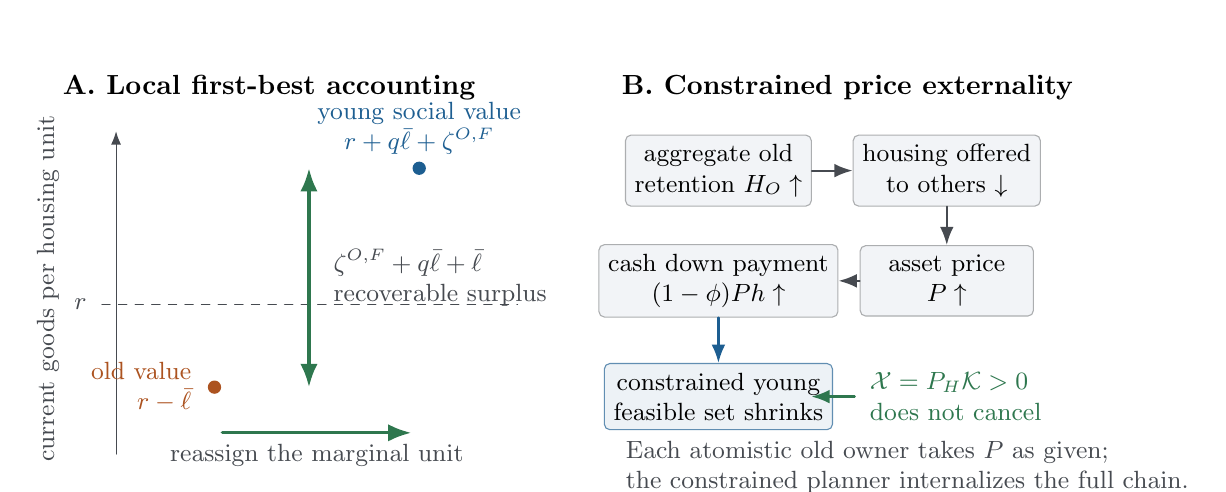
\begin{tikzpicture}[font=\small,>=Latex,line cap=round,line join=round]
% Panel A
\begin{scope}[shift={(0,0)}]
  \node[anchor=west,font=\bfseries] at (0,5.1) {A. Local first-best accounting};
  \draw[->,darkgray] (0.8,0.45) -- (0.8,4.55);
  \node[rotate=90,anchor=south,align=center,text=darkgray] at (0.20,2.55)
    {current goods per housing unit};
  \draw[darkgray,dashed] (0.62,2.35) -- (5.9,2.35);
  \node[anchor=east,darkgray] at (0.55,2.35) {$r$};
  \fill[oldorange] (2.05,1.30) circle (2.4pt);
  \fill[youngblue] (4.65,4.08) circle (2.4pt);
  \node[oldorange,anchor=east,align=right] at (1.88,1.30)
    {old value\\$r-\ellbar$};
  \node[youngblue,anchor=south,align=center] at (4.65,4.13)
    {young social value\\$r+q\ellbar+\zF$};
  \draw[<->,very thick,plannergreen] (3.25,1.30) -- (3.25,4.08)
    node[midway,right=5pt,align=left,text=darkgray]
    {$\zF+q\ellbar+\ellbar$\\recoverable surplus};
  \draw[->,very thick,plannergreen] (2.15,0.72) -- (4.55,0.72)
    node[midway,below,align=center,text=darkgray]
    {reassign the marginal unit};
\end{scope}

% Panel B
\begin{scope}[shift={(7.1,0)}]
  \node[anchor=west,font=\bfseries] at (0,5.1) {B. Constrained price externality};
  \tikzset{mechanism/.style={draw=darkgray!45,rounded corners=2pt,
      minimum width=2.2cm,minimum height=0.72cm,align=center,fill=softgray}}
  \node[mechanism] (ret) at (1.35,4.05) {aggregate old\\retention $H_O\uparrow$};
  \node[mechanism] (avail) at (4.25,4.05) {housing offered\\to others $\downarrow$};
  \node[mechanism] (price) at (4.25,2.65) {asset price\\$P\uparrow$};
  \node[mechanism] (cash) at (1.35,2.65) {cash down payment\\$(1-\phi)Ph\uparrow$};
  \node[mechanism,draw=youngblue!70,fill=youngblue!8] (set) at (1.35,1.18)
    {constrained young\\feasible set shrinks};
  \draw[->,thick,darkgray] (ret) -- (avail);
  \draw[->,thick,darkgray] (avail) -- (price);
  \draw[->,thick,darkgray] (price) -- (cash);
  \draw[->,thick,youngblue] (cash) -- (set);
  \node[anchor=west,align=left,text=plannergreen] at (3.15,1.18)
    {$\mathcal X=P_H\mathcal K>0$\\does not cancel};
  \draw[->,thick,plannergreen] (3.08,1.18) -- (2.53,1.18);
  \node[anchor=west,align=left,text=darkgray] at (0.05,0.28)
    {Each atomistic old owner takes $P$ as given;\\the constrained planner internalizes the full chain.};
\end{scope}
\end{tikzpicture}
\caption{Two different efficiency arguments. Panel A is a direct
first-best reassignment that bypasses mortgage access. Panel B keeps the same
underwriting rule but changes its endogenous price input through coordinated
old release. Ordinary price gains and losses cancel; the collateral-constraint
effect remains.}
\label{fig:two_efficiency_results}
\end{figure}

\subsection{Policy implementation and theorem}

To turn \eqref{eq:externality} into a Pareto statement, the policy, transfers,
prices, and demands must be solved jointly. Let $v_a(P,\tau,T_a)$ be household
$a$'s optimized lifetime utility on its fixed tenure branch when $T_a$ is an
anticipated but nonpledgeable present-value settlement. Let
$\bar U_a=v_a(P_0,0,0)$. Because $v_{a,T}>0$, the implicit equation
\begin{equation}
v_a\!\left(P,\tau,T_a^c(P,\tau;\bar U_a)\right)=\bar U_a
\label{eq:exact_cv}
\end{equation}
defines the household's exact compensating transfer locally. These transfers
are included in wealth effects and hence in demand. Define compensated
aggregate housing demand
\begin{equation}
D^c(P,\tau;\bar{\mathbf U})
=\int h_a\!\left(P,\tau,T_a^c(P,\tau;\bar U_a)\right)\,\dd M(a).
\label{eq:compensated_demand}
\end{equation}
The compensated equilibrium price $P^c(\tau)$ solves
\begin{equation}
D^c(P^c(\tau),\tau;\bar{\mathbf U})=\bar H.
\label{eq:compensated_clearing}
\end{equation}
If $D_P^c<0$ and $D_\tau^c<0$ at the baseline, the implicit-function theorem
gives
\begin{equation}
\boxed{
P_\tau^c=-\frac{D_\tau^c}{D_P^c}<0.}
\label{eq:Ptauc}
\end{equation}
This is the relevant price derivative. Replacing it by the uncompensated
derivative of \eqref{eq:residual_clearing} would be incorrect.

The sign $D_\tau^c<0$ is not mysterious in the written log problem. Set
$\ellbar=0$, let $A\equiv1+\gamma+\omega_B$, and impose a current tax $\tau$
per unit of old retained housing. At a fixed $P$, an interior old owner with
$W_j\equiv b_j+rH_j^0$ solves
\begin{equation}
c_j^2+e_j+(r+\tau)h_j^2=W_j+T_j.
\end{equation}
Hence
\begin{equation}
h_j^2=\frac{\gamma(W_j+T_j)}{A(r+\tau)}.
\end{equation}
Exact compensation implies
$\partial T_j^c/\partial\tau=h_j^2$ at the baseline. Therefore
\begin{equation}
\left.\frac{\partial h_j^{2,c}}{\partial\tau}\right|_{P,\tau=0}
=-\frac{1+\omega_B}{Ar}\,h_j^2<0.
\label{eq:old_compensated_release}
\end{equation}
Thus a positive measure of interior old owners supplies the desired direct
release. The aggregate compensated own-price slope $D_P^c<0$ remains a
regularity condition; it is not guaranteed by the household first-order
conditions when endowment and settlement effects are present.

The last object is the consolidated settlement account. Let
$\Pi^c(P,\tau)$ collect current and dated tax receipts and the net income of
passive housing, lending, and asset counterparties, all expressed in date-$t$
goods and measured relative to baseline. Define the balance left after exact
compensation,
\begin{equation}
\mathcal B^c(\tau)
=\Pi^c(P^c(\tau),\tau)
-\int T_a^c(P^c(\tau),\tau;\bar U_a)\,\dd M(a).
\label{eq:consolidated_balance}
\end{equation}

\begin{lemma}[Consolidated compensation identity]
\label{lem:compensation_identity}
Suppose every housing claimant, passive landlord, lender, and tax recipient is
inside the account; the retention tax is rebated; there are no first-order real
policy costs; and the displayed young down-payment inequalities are the only
active constraints whose feasible sets depend on $P$. Then
\begin{equation}
\left.\frac{\dd\mathcal B^c}{\dd\tau}\right|_{0}
=-P_\tau^c\mathcal K.
\label{eq:balance_envelope}
\end{equation}
\end{lemma}

\begin{proof}
Differentiate each exact-compensation equation \eqref{eq:exact_cv} and divide
by its budget multiplier. Decompose the required transfer as
\begin{equation}
\dd T_a^c
=\dd T_a^{\mathrm{ord}}
+\1\{a\in\mathcal C_O\}
 \frac{\mu_a}{\lambda_a}(1-\phi)h_a\,\dd P
+\1\{a\text{ is treated old}\}h_a^2\,\dd\tau.
\label{eq:cv_decomposition}
\end{equation}
The first term collects ordinary user-cost, asset-income, and wealth exposures.
Housing clearing and the closed ownership accounts imply that its integral is
exactly the corresponding passive-sector receipt in $\dd\Pi^c$. The last term
integrates to the first-order retention-tax revenue, also in $\dd\Pi^c$.
Those terms therefore cancel in \eqref{eq:consolidated_balance}. The middle
term integrates to $\mathcal K\dd P$: a higher price tightens a binding
down-payment inequality and requires additional compensation. Hence
$\dd\mathcal B^c=-\mathcal K\dd P$. Substituting
$\dd P=P_\tau^c\dd\tau$ proves \eqref{eq:balance_envelope}.
\end{proof}

Equation \eqref{eq:balance_envelope} is a consolidated-budget identity, not a
claim that ordinary price changes create resources. Its right side survives
because a price change alters a binding feasible set. The source note does not
write the counterpart budgets needed for the first cancellation; applying the
lemma literally therefore requires the passive-sector closure listed in
Section~\ref{sec:missing}.

\begin{proposition}[Fixed-cross-section constrained inefficiency]
\label{prop:constrained}
Set $\ellbar=0$ to isolate financing. Consider the implementation problem in
Definition~\ref{def:constrained}. Suppose: (i) the exact compensated system
\eqref{eq:exact_cv}--\eqref{eq:compensated_clearing} is locally unique and
differentiable with fixed household measures and stable tenure and entry
branches; (ii) a positive mass of young owners has $\mu_i>0$ and a slack
owner-size cap, so $\mathcal K>0$; (iii) a positive measure of treated old
owners is at an interior retention margin, $D_\tau^c<0$, and $D_P^c<0$, so
$P_\tau^c<0$; (iv) the closed-account hypotheses of
Lemma~\ref{lem:compensation_identity} hold; and (v) policy settlements are
legally nonpledgeable. Then the baseline
is locally constrained Pareto inefficient relative to that policy set. The
first-order date-$t$ consumption-equivalent surplus is
\begin{equation}
\boxed{
\left.\frac{\dd\mathcal S^C}{\dd\tau}\right|_{\tau=0}
=-P_\tau^c\mathcal K>0.}
\label{eq:constrained_surplus}
\end{equation}
Every young owner continues to satisfy the same down-payment constraint
\eqref{eq:dp_policy}.
\end{proposition}

\begin{proof}
Solve \eqref{eq:exact_cv} and \eqref{eq:compensated_clearing} jointly. Thus
every household is held at its baseline lifetime utility, while anticipated
settlements and their income effects are already incorporated in
$P^c(\tau)$. For a constrained young owner, the compensating-transfer effect
of a price change through \eqref{eq:dp_policy} is
\[
+\frac{\mu_i}{\lambda_i}(1-\phi)h_i\,\dd P.
\]
The sign is positive because a price increase requires additional compensation
when the constraint tightens. Summing gives $\mathcal K\dd P$ as a cost to the
consolidated settlement account. The compensated retention-tax cost is exactly
offset by tax revenue at first order, and ordinary price exposures cancel by
the closed-account assumption. Along the equilibrium path
$\dd P=P_\tau^c\dd\tau$, so the net balance derivative is
$-P_\tau^c\mathcal K>0$, as in \eqref{eq:balance_envelope}.

For sufficiently small $\tau>0$, exact compensation of every baseline utility
therefore leaves a strictly positive consolidated balance. Raise one
household's target utility by a sufficiently small amount and resolve the same
compensated system. Local nonsatiation and regularity imply that this uses less
than the positive balance, leaving every other household at baseline utility.
This is a finite Pareto improvement. Throughout the path, transfers remain
nonpledgeable and each optimized choice satisfies \eqref{eq:dp_policy}; the
constraint relaxes only because its endogenous price coefficient falls.
\end{proof}

The corresponding old-retention conditions summarize the economics. Let
$P_H^c>0$ be the response to a compensated coordinated increase in aggregate
old retention and define $\mathcal X^c=P_H^c\mathcal K$. Without
the gains tax, an atomistic old owner retains housing until
\begin{equation}
\MRS_j^O=r.
\label{eq:old_private_notax}
\end{equation}
The constrained planner internalizes the collateral effect and instead uses
\begin{equation}
\MRS_j^O=r+\mathcal X^c.
\label{eq:old_planner_constrained}
\end{equation}
Because marginal utility of housing falls with retained housing, the planner
chooses less old retention. With an existing gains tax and a locally fixed
$\ellbar$, the private condition is $\MRS_j^O=r-\ellbar$, so the old-retention
gap becomes $\mathcal X^c+\ellbar$. A local Pigouvian tax on retained housing
is therefore $\tau^{H,*}=\mathcal X^c$ when $\ellbar=0$, and
$\tau^{H,*}=\mathcal X^c+\ellbar$ when the existing sale tax is held fixed.
The buyer's anticipated $q\ellbar$ is a separate ownership-timing wedge. In a
general-equilibrium tax reform it should not be appended mechanically: its
contribution depends on which tenure absorbs released housing, whether
$\ellbar$ moves with $P$, and the fiscal closure.

\subsection{Why stronger constrained claims fail}

Three counterexamples discipline the theorem.

\textbf{Exogenous price.} Suppose outside supply is perfectly elastic at
$P=\bar P$. A young owner's down-payment constraint may bind with
$\mu_i>0$, but $P_H=0$ and hence $\mathcal X=0$. If the constrained planner
cannot transfer pledgeable wealth before underwriting, it cannot increase the
young household's feasible owner housing. A binding constraint can coexist
with constrained efficiency.

\textbf{No constrained exposure.} If all $\mu_i=0$, then $\mathcal K=0$.
Old retention can raise $P$, but this is an ordinary pecuniary effect: gains to
sellers and losses to buyers can be redistributed without changing anyone's
feasible set.

\textbf{Wrong price response or real costs.} If aggregate demand is not locally
downward sloping, if the policy fails to reduce retention, or if the marginal
administrative, moving, or conversion cost exceeds
$-P_\tau^c\mathcal K$, the sign in \eqref{eq:constrained_surplus} is not
positive. The theorem is conditional on an economic response that must be
derived or estimated, not asserted.

\textbf{Offsetting price-dependent constraints.} Suppose a lower $P$ relaxes
the displayed young down-payment caps but tightens an intermediary's solvency
constraint or another household's collateral limit. Its multiplier-weighted
envelope term must be added to $\mathcal K$ with the appropriate sign. The
financing result can disappear or reverse. This is why
Proposition~\ref{prop:constrained} either excludes such constraints or requires
their complete accounting.

\textbf{Stationary-comparison fallacy.} A permanent change in $P$ changes
future states, entry, tenure, tax bases, and possibly population. A comparison
of two stationary cross-sections is not a Pareto comparison among a fixed set
of people. Proposition~\ref{prop:constrained} is deliberately a one-date
implementation result. A permanent-policy theorem requires a transition path
and the sum of every active constraint envelope at every date.

% ================================================================
\section{Discrete tenure transitions}
\label{sec:tenure}
% ================================================================

Young tenure is discrete. A derivative taken inside the owner branch does not
prove that a renter should become an owner, and a derivative taken inside the
renter branch does not price the fixed change in continuation values and
financial feasibility at a tenure switch.

Let $\mathbf m$ denote the vector of tenure assignments. For a target vector of
lifetime utilities $\bar{\mathbf U}$, the general branch comparison is between
feasible utility sets,
\begin{equation}
\mathcal U(\mathbf m)
=\left\{\mathbf U:\ \exists x\in\mathcal F(\mathbf m)
\text{ with }U_a(x)\ge U_a\ \forall a\right\}.
\label{eq:branch_utility_set}
\end{equation}
Only if dated goods are freely transferable through complete claims at the
stated prices can this comparison be reduced to a scalar present-value
expenditure function. Under that additional assumption, define
\begin{equation}
\mathcal E(\mathbf m;\bar{\mathbf U})
=\inf_{x\in\mathcal F(\mathbf m)}
\left\{\sum_{t\ge0}q^t \mathcal R_t^{\mathrm{real}}(x):
U_a(x)\ge\bar U_a\ \text{for every household }a\right\},
\label{eq:branch_expenditure}
\end{equation}
where $\mathcal F(\mathbf m)$ contains the physical housing, goods, and
implementation constraints appropriate to the planner under study, and
$\mathcal R_t^{\mathrm{real}}(x)$ counts only real resources. House purchases,
rents, principal, and rebated taxes are excluded.

\begin{proposition}[Finite tenure criterion]
\label{prop:finite_tenure}
Let $\mathbf m^0$ be the competitive tenure vector and
$\bar{\mathbf U}$ its utility vector. In general, a tenure change to
$\mathbf m^1$ supports a Pareto improvement if and only if there is an
$x^1\in\mathcal F(\mathbf m^1)$ such that
\begin{equation}
U_a(x^1)\ge\bar U_a\quad\forall a,
\qquad
U_k(x^1)>\bar U_k\quad\text{for some }k.
\label{eq:finite_feasible_test}
\end{equation}
If complete intertemporal claims permit scalar present-value accounting,
resource endowments are common across branches, free disposal holds, and the
infima are attained, the sufficient expenditure test is
\begin{equation}
\mathcal E(\mathbf m^1;\bar{\mathbf U})
<\mathcal E(\mathbf m^0;\bar{\mathbf U}).
\label{eq:finite_tenure_test}
\end{equation}
The resource difference can then be given to one household after everyone is
held at baseline utility. Without complete dated claims, use
\eqref{eq:finite_feasible_test}; a future resource saving cannot automatically
finance a current shortfall. If no lotteries or convexification are allowed,
these finite comparisons, not a branch derivative, are the appropriate welfare
tests.
\end{proposition}

A renter-to-owner comparison must include the entire change in the young
budget branch, the down-payment feasibility test, the carried old-owner state,
future tax exposure, and the housing released by others. An owner-to-renter
comparison must do the reverse. The simplified old problem does not permit a
genuine old owner-to-renter transition; adding one requires an old tenure
choice $m_j^2\in\{R,O\}$ and a rental branch with its own budget and size set.
That is a model extension, not a proof refinement.

% ================================================================
\section{Full planner, resource accounting, and decentralization}
\label{sec:planner}
% ================================================================

The current note can write a conditional planner at a fixed cross-section. It
cannot, without additional primitives, rank allocations that jointly change
fertility, the future population, entry wealth, and the identity of future
households. This section writes a \emph{planner template under added closure
assumptions}. It is not a theorem of the current simplified model. Every object
that must be added is marked explicitly.

\subsection{A minimal dynamic-completion template}

Let $M_t(\dd i)$ be the measure of potential young types at date $t$. Let
$d_{it}^E\in\{0,1\}$ denote entry and $m_{it}\in\{R,O\}$ tenure conditional on
entry. A cohort born at $t$ receives lifetime utility
\begin{equation}
U_{it}=d_{it}^E\left[u_i^Y(c_{it},h_{it},n_{it})
+\beta u_i^O(c_{i,t+1}^2,h_{i,t+1}^2,e_{i,t+1})\right]
+(1-d_{it}^E)\bar W^E.
\label{eq:cohort_utility}
\end{equation}
The completion must specify welfare weights $\omega_{it}>0$ for every cohort
and a calendar discount factor $\Delta$. Counting each cohort once, plus the
initial old, gives the following objective. Let $M_{-1}^O(\dd j)$ be the
initial-old measure and $\omega_{j,-1}^O>0$ its welfare weights, and define
$W_{-1}^O=\int\omega_{j,-1}^O u_j^O\,M_{-1}^O(\dd j)$. Then
\begin{equation}
\max\quad
W_{-1}^O+
\sum_{t=0}^{\infty}\Delta^t
\int \omega_{it}U_{it}\,M_t(\dd i).
\label{eq:planner_objective}
\end{equation}
If entry taste shocks are structural welfare objects, they must be integrated
inside $U_{it}$; if they are only a smoothing device, the planner should not
count them. The current note does not choose between these interpretations.

Let $A_t$ be the payoff on the economy's net external bond position and
$A_{t+1}$ the next payoff purchased at price $q_t$. Let $I_t$ be housing
investment and $\Psi(I_t,H_t)$ its real resource cost. Define final domestic
goods use
\begin{equation}
C_t=
\int d_{it}^E c_{it}\,M_t(\dd i)
+\int d_{i,t-1}^E(c_{i,t}^2+e_{i,t})\,M_{t-1}(\dd i).
\end{equation}
At $t=0$, the second integral is taken directly over $M_{-1}^O$ and its
predetermined states.
Treating the warm-glow estate as a terminal delivery outside the modeled
descendant sector, the date-$t$ goods constraint is
\begin{equation}
C_t+\Psi(I_t,H_t)+q_tA_{t+1}
\le
\int d_{it}^E y_{it}\,M_t(\dd i)+A_t+Y_t^{\mathrm{outside}}.
\label{eq:planner_goods}
\end{equation}
The initial condition $A_0$ must contain the real external counterpart of
initial young wealth, initial old assets, and passive-sector equity after all
internal claims are netted. Individual $b_i$ is not itself an aggregate
resource when it is another domestic agent's liability. Let
$Q_{0,t}=\prod_{s=0}^{t-1}q_s$. Feasibility also requires a no-Ponzi condition,
for example
\begin{equation}
\liminf_{T\to\infty}Q_{0,T+1}A_{T+1}\ge0,
\label{eq:no_ponzi}
\end{equation}
with the corresponding transversality equality at an interior optimum. The
source note specifies neither $A_0$ nor this terminal condition.
If estates instead finance entrants, $e_{i,t}$ must be removed from terminal
use and linked to the next generation's asset endowment by an explicit transfer
identity.

The physical housing constraints are
\begin{align}
&\int d_{it}^E h_{it}\,M_t(\dd i)
+\int d_{i,t-1}^E h_{i,t}^2\,M_{t-1}(\dd i)
\le H_t,
\label{eq:planner_housing}\\
&H_{t+1}=(1-\delta)H_t+I_t.
\label{eq:stock_law}
\end{align}
The fixed-stock version sets $H_t=\bar H$ and therefore requires replacement
$I_t=\delta\bar H$, unless $\delta$ is reinterpreted as zero or as maintenance
already supplied by an outside endowment. The current note puts $\delta$ in
the private user cost but does not write this real resource requirement.

The population law must also be explicit. One possible closure is
\begin{align}
M_{t+1}(A)
&=\int
\left[d_{it}^E n_{it}+(1-d_{it}^E)\bar n_i^E\right]
\Gamma_Y(A\mid i,m_{it},n_{it},e_t)\,M_t(\dd i)
\notag\\
&\qquad+\mathcal R_t^{\mathrm{renew}}\Upsilon(A)
\label{eq:population_law}
\end{align}
for every measurable type set $A$. A fixed-mass housing-efficiency benchmark
instead lets $\mathcal R_t^{\mathrm{renew}}$ adjust so that $M_t$ is unchanged. Allowing fertility to
change $M_{t+1}$ requires a population-ethics choice through
$\omega_{i,t+1}$ and $\Delta$, not just more algebra.

The tenure and carried-housing restrictions complete physical feasibility:
\begin{equation}
h_{it}\le\bar h^{m_{it}},\qquad
0<h_{i,t+1}^2\le h_{it}\ \text{for a young owner},\qquad
0<h_{i,t+1}^2\le\bar h^R\ \text{for a young renter}.
\label{eq:planner_tenure_constraints}
\end{equation}
Whether $\bar h^R$ and $\bar h^O$ are physical constraints that the planner
must respect or market-access restrictions it can undo must be declared.

\subsection{Asset trades are not resource costs}

House purchases $P_tx$, rents $r_th$, mortgage advances, principal repayment,
interest receipts, property taxes, gains taxes, and lump-sum rebates do not
appear in \eqref{eq:planner_goods} after the corresponding buyers, sellers,
landlords, lenders, and government are consolidated. They redistribute claims
to goods. The real terms are final consumption, construction or replacement,
maintenance, moving/conversion/foreclosure costs, and net purchases of goods
from outside the economy.

This distinction does not mean that $P$ is irrelevant. It is irrelevant to the
first-best physical resource constraint, but it remains central to a
constrained implementation problem because $P$ enters
$(1-\phi)Ph\le b$.

\subsection{Planner conditions}

At a fixed population and on a fixed tenure branch, let $\Lambda_t$ and
$\Nu_t$ be the multipliers on goods and housing feasibility, and define the
social scarcity price
\begin{equation}
Q_t\equiv\frac{\Nu_t}{\Lambda_t}.
\end{equation}
Thus $\Lambda_t$ is planner-objective units per date-$t$ good, $\Nu_t$ is
planner-objective units per housing unit at $t$, and $Q_t$ is date-$t$ goods
per housing unit. The carry and size multipliers below have the same units as
$\Nu_t$ after the common population-density normalization.
The ownership carry restriction in \eqref{eq:planner_tenure_constraints}
cannot be imposed and then ignored in the first-order conditions. Let
$\varrho_{i,t+1}\ge0$ be its multiplier, written on
$h_{it}-h_{i,t+1}^2\ge0$, and let $\sigma_{it}^Y\ge0$ be the multiplier on the
young physical size cap. For an owner with interior consumption and housing,
the conditions are
\begin{align}
\frac{u_{h,it}^Y}{u_{c,it}^Y}
&=Q_t-\frac{\varrho_{i,t+1}}{\Lambda_t}
  +\frac{\sigma_{it}^Y}{\Lambda_t},
\label{eq:planner_h_young}\\
\frac{u_{h,i,t+1}^O}{u_{c,i,t+1}^O}
&=Q_{t+1}+\frac{\varrho_{i,t+1}}{\Lambda_{t+1}}.
\label{eq:planner_h_old}
\end{align}
An extra unit assigned to the young owner relaxes the future carry cap, while
an extra unit retained when old uses that same capacity; this explains the
opposite signs. If a first-best planner can reassign ownership freely across
dates, the individual carry restriction should be deleted and
$\varrho_{i,t+1}=0$. If it is retained but slack, and the young size cap is
also slack, the familiar equalities to $Q_t$ and $Q_{t+1}$ follow. Neither the
private down-payment multiplier nor the capital-gains tax appears in these
first-best conditions: one is an implementation constraint and the other is a
transfer.

With no direct social value of additional people and a fixed future type
measure, the young fertility condition can be written
\begin{equation}
\boxed{
\frac{\vartheta(c_{it}-\chi n_{it})}{n_{it}}
=\chi+\kappa\frac{u_{h,it}^Y}{u_{c,it}^Y}.}
\label{eq:planner_fertility}
\end{equation}
Using \eqref{eq:planner_h_young}, the last term equals
$\kappa[Q_t-\varrho_{i,t+1}/\Lambda_t+
\sigma_{it}^Y/\Lambda_t]$; it reduces to $\kappa Q_t$ only when both
ownership and size multipliers vanish.
If fertility changes future population, \eqref{eq:planner_fertility} acquires
the co-state value of the induced measure change:
\begin{equation}
\omega_{it}u_{n,it}^Y
+\Delta\left\langle \mathcal V_{t+1},
\frac{\partial M_{t+1}}{\partial n_{it}}\right\rangle=0.
\label{eq:fertility_costate}
\end{equation}
The simplified model does not define $\mathcal V_{t+1}$, because it does not
close population welfare or the mapping from estates to entrants.

\subsection{Decentralization}

The current note cannot support a decentralization proposition because the
budgets needed to verify one are missing. The following are
\emph{decentralization conditions for a completed model}, not assumptions that
can substitute for proving the theorem:
\begin{enumerate}
\item Specify every household, landlord, lender, construction firm,
government, and external-asset budget, together with ownership of profits and
the initial claims summarized by $A_0$.
\item Require market clearing, government budget balance, zero-profit or
ownership conditions, and \eqref{eq:no_ponzi}; verify that they aggregate to
\eqref{eq:planner_goods}--\eqref{eq:stock_law}.
\item Provide complete date- and state-contingent claims, or list every missing
insurance market. Match $q_t$ and the housing user cost to the planner's goods,
intertemporal, stock, and carry co-states.
\item Remove or correctly price all wedges: financing constraints, differential
sale-versus-retention taxation, unpriced maintenance or supply restrictions,
and any entry, fertility, population, or bequest externality.
\item Treat discrete tenure explicitly. Convexity is not required for the
first welfare theorem itself, but it matters for supporting arbitrary planner
allocations and for derivative-based sufficiency; lotteries are one possible
convexification.
\end{enumerate}
After those objects are specified, the standard first-welfare logic implies
that a competitive equilibrium with locally nonsatiated preferences and no
unpriced wedges is Pareto efficient. House purchases and mortgages then merely
transfer asset claims. That conditional statement is economically useful, but
it is not a theorem of the displayed simplified model.

In particular, removing financing constraints alone is insufficient if
$\ellbar>0$ continues to distort release, if claims are incomplete, or if
fertility and entry have unpriced population effects. If all such wedges are
also absent or correctly priced, the completed competitive equilibrium is
efficient. With $\ellbar=0$ but binding finance, Corollary~\ref{cor:no_tax}
gives the first-best result when the planner bypasses the cap, while
Proposition~\ref{prop:constrained} gives the narrower fixed-cross-section
constrained result only under its compensated-equilibrium conditions.

% ================================================================
\section{What is missing from the current model}
\label{sec:missing}
% ================================================================

Most of what is needed for the first-best theorem is proof apparatus, not a new
economic mechanism. The constrained theorem uses the note's existing mechanism
---endogenous $P$, old retention, a fixed stock, market clearing, and the
down-payment inequality---but it also needs a minimal implementation closure.
Specifically, it requires:
\begin{enumerate}
\item a one-date, fixed-cross-section definition of constrained implementation;
\item exact anticipated compensating transfers that are nonpledgeable but are
included in household demand;
\item a jointly solved compensated price response $P_\tau^c$, not the
uncompensated derivative of ordinary demand;
\item a policy or coordinated retention perturbation and its transfer timing;
\item consolidated fiscal and passive-sector accounts sufficient to establish
\eqref{eq:balance_envelope}; and
\item an explicit restriction excluding offsetting price-dependent constraints,
or a complete sum of their multiplier-weighted envelope effects.
\end{enumerate}

A literal full planner and a literal mortgage interpretation require actual
model closures:
\begin{itemize}
\item \textbf{Mortgage balance sheet.} Introduce down-payment equity $E_i$ and
debt $D_i$ with
\[
P h_i=E_i+D_i,\qquad E_i\le b_i,\qquad D_i\le\phi P h_i,
\]
and track purchase, debt service, resale, and terminal equity explicitly. This
prevents the same liquid wealth from both being posted at closing and remaining
fully spendable.
\item \textbf{Fiscal closure.} State who receives property- and gains-tax
revenue, when it is rebated, and whether the planner can transfer resources
across dates at $q$.
\item \textbf{Passive sectors.} State ownership of landlords, lenders, and the
outside bond position so that price changes and payments can be consolidated.
\item \textbf{Housing technology.} Add a stock law and the real cost of
maintenance/replacement, or set $\delta=0$ in the fixed-stock analytical model.
\item \textbf{Bequests and entry wealth.} Either link $e_j$ to the distribution
of future $b_i$, or declare estates a terminal good delivered outside the
modeled population.
\item \textbf{Outside option and population ethics.} Specify the outside
option's resource use, outside fertility, the renewal law, and welfare weights
on future people before asking the planner to vary entry and fertility.
\item \textbf{Old tenure transition.} Add an old renter branch for incumbents
if ``sell and rent'' is intended to be a discrete margin rather than continuous
downsizing within ownership.
\end{itemize}

These omissions do not invalidate the local accounting if the access-cap and
fiscal interpretations are stated. They do prevent the current equations from
supporting an unconditional theorem over housing, consumption, saving,
fertility, tenure, entry, and intergenerational allocation.

% ================================================================
\section{Audit of the existing proposition and proof}
\label{sec:audit}
% ================================================================

\begin{center}
\renewcommand{\arraystretch}{1.17}
\begin{tabularx}{\textwidth}{@{}L{0.30\textwidth}Y@{}}
\toprule
Existing step & Audit \\
\midrule
``Hold the stationary cross-section, entry, tenure assignments, and savings
fixed.''
& Appropriate for a conditional local result, but ``stationary'' is stronger
than needed. The dynamic path of the marginal unit must be stated: the young
owner carries it, the planner holds her future retained quantity fixed, and
the added unit is sold next period. Interiority makes this constructed path
first-order equivalent to reoptimization; it does not imply one-for-one sale
by itself. \\
``Move one unit.''
& The theorem is marginal. Write $\varepsilon>0$ and use continuity to obtain a
finite local Pareto improvement. A literal unit need not be small. \\
Buyer value $r^O+\zeta^{O,F}$ with $r^O=r+q\ellbar$.
& Correct as the current static MRS for an interior saver. More generally the
static MRS uses $d_i\ellbar$. It is not the buyer's private lifetime WTP, which
is $r+\zeta^{O,F}$. \\
Old value $r-\ellbar$.
& Correct only at an interior retention margin. At $h^2=H^0$, use a
Kuhn--Tucker inequality and the sign need not follow. \\
Subtract to obtain $\zeta^{O,F}+q\ellbar+\ellbar$.
& Correct under the fiscal closure. The same expression follows from private
lifetime WTP plus the future fiscal receipt. It is not a duplicated purchase
price. \\
``Taxes are transfers.''
& Requires government receipts and rebates inside the social boundary. If
revenue leaves the jurisdiction or is destroyed, the formula changes. \\
``Compensate the incumbent.''
& Incomplete as written. The rigorous construction also charges the young
household her financing surplus and tracks current and future tax receipts.
Proposition~\ref{prop:local} supplies the exact compensated variation. \\
``The competitive allocation does not solve the planner problem.''
& Correct for the conditional first-best problem. It does not establish
constrained inefficiency when the planner must respect the same fixed-price
down-payment inequality. Proposition~\ref{prop:constrained} is the separate
constrained theorem. \\
``Compensate price losers and use $P_\tau$.''
& Incomplete unless the compensating transfers are included in household
demand. The relevant object is $P_\tau^c$ from
\eqref{eq:exact_cv}--\eqref{eq:compensated_clearing}; anticipated transfers
change both retention and residual demand. \\
\bottomrule
\end{tabularx}
\end{center}

% ================================================================
\section{Proposed replacement subsection for the paper}
\label{sec:replacement}
% ================================================================

The text below is designed to be copied into the paper after notation is
harmonized with the surrounding section. It separates the first-best and
constrained results and makes the fiscal accounting explicit.

\vspace{0.4em}
\hrule
\vspace{0.6em}

\subsection*{Housing allocation and efficiency}

We distinguish two welfare questions. A first-best planner allocates the
existing housing stock and can bypass private mortgage access. An
equilibrium-constrained planner must instead implement allocations through the
same down-payment rule households face, evaluated at the price generated by
the policy equilibrium. The first question delivers a direct marginal
reallocation result; the second isolates a collateral pecuniary externality.

For the local first-best comparison, consolidate passive landlords, lenders,
and the government, and rebate tax revenue lump sum. House purchases, rents,
mortgage principal, and tax payments are then transfers rather than resource
costs. The planner faces the fixed housing stock and any physical size or
conversion constraints, but not the private down-payment inequality. We use a
marginal unit with zero real reallocation cost.

At an interior old retention choice, the old-owner problem implies
\begin{equation}
\frac{u_{h,j}^O}{u_{c,j}^O}=r-\ellbar,
\qquad
V_H^O=(r-\ellbar)V_b^O.
\label{eq:paper_old_margin}
\end{equation}
For a young owner, let $\lambda_i$ and $\mu_i$ be the multipliers on the
current budget and down-payment constraint, and define the financing wedge in
current consumption units,
\begin{equation}
\zeta_i^{O,F}=\frac{\mu_i}{\lambda_i}(1-\phi)P.
\label{eq:paper_finance_wedge}
\end{equation}
If the owner-size limit is slack, the housing condition and
\eqref{eq:paper_old_margin} imply
\begin{equation}
\frac{u_{h,i}^Y}{u_{c,i}^Y}
=r+d_i\ellbar+\zeta_i^{O,F},
\qquad
d_i\equiv\frac{\beta V_b^O}{\lambda_i}.
\label{eq:paper_young_margin}
\end{equation}
For an interior saver, $d_i=q$. The household's private lifetime willingness
to pay nets out the continuation loss from the future tax and equals
$r+\zeta_i^{O,F}$. The fiscal-inclusive social value adds back the date-$t$
value $q\ellbar$ of the future tax receipt.

\begin{proposition}[Local reallocation]
Suppose young owner $i$ has a slack physical size limit and a binding
down-payment constraint, current old owner $j$ is at an interior release
margin, and the young owner's future retention choice is interior. Consider a
path that holds the young owner's future retained housing fixed and releases
the additional carried unit. If housing is divisible, the marginal unit has no
real reassignment cost, and current and future tax revenue is rebated, then
moving a marginal unit from $j$ to $i$ generates consumption-equivalent surplus
\begin{equation}
\zeta_i^{O,F}+q\ellbar+\ellbar>0.
\label{eq:paper_local_surplus}
\end{equation}
The competitive allocation is therefore locally Pareto inefficient relative
to a planner that can bypass mortgage access. With $\ellbar=0$, the surplus is
$\zeta_i^{O,F}>0$; financing alone is sufficient.
\end{proposition}

\begin{proof}
Let the old owner release $\varepsilon$ units with the flow-equivalent
settlement $r\varepsilon$.
She nets $r-\ellbar$ per unit, exactly her marginal value by
\eqref{eq:paper_old_margin}, and is unchanged to first order; the government
receives $\ellbar\varepsilon$. Let the young owner acquire the unit while
holding fertility and saving fixed. After the market payment, her lifetime
utility rises by
$\lambda_i\zeta_i^{O,F}\varepsilon+o(\varepsilon)$, so a lump-sum settlement
charge $\zeta_i^{O,F}\varepsilon+o(\varepsilon)$ holds her indifferent. At
date $t+1$, hold her retained housing fixed, reduce old consumption and the
estate by a total $\ellbar\varepsilon$ in their conditional
expenditure-minimizing shares, and release the added carried unit. This is
first-order equivalent to reoptimization because future retention is interior,
and it produces exactly one additional taxable sale, with present value
$q\ellbar\varepsilon$. The planner is left with
$[\zeta_i^{O,F}+\ellbar+q\ellbar]\varepsilon+o(\varepsilon)$ goods. For
sufficiently small $\varepsilon$, assigning the positive residual to one
household is a Pareto improvement.
\end{proof}

The explicit future path matters. Interiority alone does not imply that an
unrestricted old household sells exactly the additional unit: future retained
housing generally reoptimizes with the tax base. The envelope theorem is what
permits the fixed-retention construction without a first-order private utility
loss.

The proposition is first best: the planner places a unit that the buyer cannot
privately finance. To ask whether the equilibrium is inefficient subject to
the same mortgage rule, let aggregate old retention be $H_O$ and write residual
housing demand as $D_{-O}(P)$. Market clearing gives
$D_{-O}(P)+H_O=\bar H$. If $D_{-O}'(P)<0$, aggregate old retention raises the
price,
\begin{equation}
P_H=-\frac{1}{D_{-O}'(P)}>0.
\label{eq:paper_price_response}
\end{equation}
Because the price enters the cash-at-closing requirement, the goods-equivalent
collateral cost of one more unit of old retention is
\begin{equation}
\mathcal X
=P_H\int_{\mathcal C_O}
\frac{\mu_i}{\lambda_i}(1-\phi)h_i\,\dd M_Y(i)
=\frac{P_H}{P}\int_{\mathcal C_O}
\zeta_i^{O,F}h_i\,\dd M_Y(i).
\label{eq:paper_externality}
\end{equation}
An atomistic old owner takes $P$ as given and does not internalize
\eqref{eq:paper_externality}.

For a Pareto theorem, compensating transfers must be included in demand. Fix
the current population, states, entry decisions, and tenure branches. Let
$v_a(P,\tau,T_a)$ be household $a$'s optimized lifetime utility when $\tau$ is
a tax on current old retention and $T_a$ is an anticipated, nonpledgeable
settlement. Define $T_a^c$ by
\begin{equation}
v_a(P,\tau,T_a^c)=\bar U_a,
\end{equation}
and let $D^c(P,\tau;\bar{\mathbf U})$ be aggregate housing demand evaluated at
these exact compensating settlements. The jointly compensated equilibrium
price satisfies
\begin{equation}
D^c(P^c(\tau),\tau;\bar{\mathbf U})=\bar H,
\qquad
P_\tau^c=-\frac{D_\tau^c}{D_P^c}.
\label{eq:paper_compensated_price}
\end{equation}
The ordinary, uncompensated price derivative is not the relevant object.

\begin{proposition}[Constrained inefficiency from old retention]
Set $\ellbar=0$ to isolate financing. Suppose: (i) a positive mass of young
owners has binding down-payment constraints; (ii) the exact compensated
equilibrium is locally unique with stable entry and tenure branches;
(iii) $D_\tau^c<0$ and $D_P^c<0$, so $P_\tau^c<0$; (iv) landlords, lenders,
housing claimants, and government are inside a closed settlement account;
(v) the down-payment inequalities are the only active price-dependent
constraints with a nonzero aggregate envelope term; and (vi) policy and
reallocation have no first-order real cost. Then the fixed-cross-section
baseline is locally constrained Pareto inefficient. Along the policy
equilibrium, all young owners continue to satisfy
$(1-\phi)P^c(\tau)h_i(\tau)\le b_i$, and the first-order compensated surplus is
\begin{equation}
\left.\frac{\dd\mathcal S^C}{\dd\tau}\right|_{\tau=0}
=-P_\tau^c
\int_{\mathcal C_O}
\frac{\mu_i}{\lambda_i}(1-\phi)h_i\,\dd M_Y(i)>0.
\label{eq:paper_constrained_surplus}
\end{equation}
\end{proposition}

\begin{proof}
Solve the compensation equations and housing clearing jointly, so all wealth
effects of $T_a^c$ are already incorporated in $P^c(\tau)$. At the baseline,
the direct compensating cost of the retention tax equals its tax revenue.
Ordinary price exposures cancel in the closed account. A price increase,
however, raises the transfer required to compensate constrained young owner
$i$ by
$[\mu_i/\lambda_i](1-\phi)h_i\,\dd P$. Therefore the consolidated balance
after holding every household at $\bar U_a$ has derivative equal to the right
side of \eqref{eq:paper_constrained_surplus}. It is strictly positive because
$P_\tau^c<0$. For a sufficiently small positive tax, use part of the residual
to raise one target utility and resolve the compensated equilibrium. Every
other utility remains at baseline and every down-payment inequality is
satisfied at the new price, establishing a constrained Pareto improvement.
\end{proof}

For the old log problem, the direct compensated release condition is readily
checked. With $A=1+\gamma+\omega_B$ and an interior old owner,
\begin{equation}
\left.\frac{\partial h_j^{2,c}}{\partial\tau}\right|_{P,\tau=0}
=-\frac{1+\omega_B}{Ar}h_j^2<0.
\end{equation}
Thus the nontrivial aggregate assumption is the compensated own-price slope
$D_P^c<0$. A permanent-policy or stationary-equilibrium claim would require a
full transition and all future constraint envelopes; the proposition above is
deliberately a one-date result for a fixed set of households.

The constrained result is not implied by a binding constraint alone. If house
prices are exogenous, then $P_H=0$ and the collateral externality vanishes. If
all financing multipliers are zero, a price change is purely pecuniary. With an
existing capital-gains tax, old owners privately retain until
$u_h^O/u_c^O=r-\ellbar$. Let
$\mathcal X^c=P_H^c\mathcal K$ use the compensated price response to a
coordinated retention change. The constrained planner's opportunity cost is
$r+\mathcal X^c$, so the old-retention wedge is
$\ellbar+\mathcal X^c$. The buyer's anticipated $q\ellbar$ remains a distinct
ownership-timing wedge and should be included in a general policy theorem only
after specifying which tenure absorbs released housing and how tax liabilities
move with $P$.

\vspace{0.6em}
\hrule

% ================================================================
\appendix
\section{Corner cases and robustness}

\textbf{Young saving corner.} If $b_i'=0$, then $d_i<q$ in
\eqref{eq:young_static_mrs}. The private lifetime value
$r+\zeta_i^{O,F}$ remains the correct envelope object. A fiscal-inclusive
planner that can trade at $q$ still values a future tax receipt at $q\ellbar$,
but the current static MRS is no longer $r+q\ellbar+\zeta_i^{O,F}$.

\textbf{Old retention corner.} If $h_j^2=H_j^0$, the old MRS is weakly above
$r-\ellbar$. A small release may still be desirable, but the exact gap must use
the old household's actual one-sided MRS. If the young owner's future old self
also keeps the entire marginal unit, no future tax is generated and the
$q\ellbar$ term is absent.

\textbf{Tax revenue outside the planner boundary.} If only a share
$\sigma_G\in[0,1]$ of tax receipts is rebated to households the planner counts,
replace $q\ellbar+\ellbar$ in the fiscal surplus by
$\sigma_G(q\ellbar+\ellbar)$, while accounting for any real collection cost.

\textbf{Endogenous tax base.} Because \eqref{eq:gains_tax} makes
$\ellbar$ proportional to $P$, a general-equilibrium policy derivative contains
terms in $\dd\ellbar/\dd P$. The fixed-price local proposition holds
$\ellbar$ constant. The constrained finance-only theorem sets $\ellbar=0$ to
avoid mixing the collateral externality with endogenous tax-base effects.

\textbf{Owner size cap.} If $\bar h^O$ binds, the young marginal gap includes
$\zeta_i^{O,S}$. Whether that term is an inefficiency depends on whether the cap
is a physical feature the planner must respect or a removable market-access
restriction. It should not be relabeled a financing wedge.

\textbf{Discrete housing.} If the marginal house cannot be divided, replace
all derivative tests with the finite compensating-expenditure comparison in
Proposition~\ref{prop:finite_tenure}. The sign of a local continuous wedge need
not dominate a fixed moving, tenure, or mismatch cost.

\section{Independent algebra and finite-difference checks}

The envelope identities can be checked without using any proposition. Set
$r=1$, $\ellbar=0.2$, $\gamma=\omega_B=1$, $b=1$, and $H^0=2$. Then
$A=1+\gamma+\omega_B=3$, total old resources are
$W=b+(r-\ellbar)H^0=2.6$, and the interior optimum is
$c^2=e=0.866\overline6$ and $h^2=1.083\overline3<H^0$. The closed-form value
function gives
\begin{equation}
V_b=\frac{A}{W}=1.153846\ldots,
\qquad
V_H=(r-\ellbar)\frac{A}{W}=0.923077\ldots,
\qquad
\frac{V_H}{V_b}=0.8=r-\ellbar.
\end{equation}
A central difference with step $10^{-5}$ gives respectively
$1.153846153856$ and $0.923076923054$; both absolute errors are below
$2.4\times10^{-11}$.

For $q=0.9$ and $\zeta^{O,F}=0.25$, the three independently derived housing
values are
\begin{center}
\renewcommand{\arraystretch}{1.12}
\begin{tabular}{@{}lcc@{}}
\toprule
Object & Formula & Value \\
\midrule
Old retention value & $r-\ellbar$ & $0.80$ \\
Young current static MRS & $r+q\ellbar+\zeta^{O,F}$ & $1.43$ \\
Young private lifetime WTP & $r+\zeta^{O,F}$ & $1.25$ \\
Fiscal-inclusive local gap & $\zeta^{O,F}+q\ellbar+\ellbar$ & $0.63$ \\
\bottomrule
\end{tabular}
\end{center}
Finally, unrestricted future reoptimization would change the taxable release
base at rate
\begin{equation}
1+\frac{\gamma\ellbar}{A(r-\ellbar)}=1.083\overline3,
\end{equation}
not one. This numerical check is the reason the proof specifies the
fixed-retention future path rather than inferring it from interiority.

\section{Assumption checklist for a paper theorem}

Before citing either proposition, the paper should state:
\begin{enumerate}
\item whether $P$ is an asset price and $r$ a one-period housing-service price;
\item that $q$ prices next-period consumption and $q\ellbar$ is a present value;
\item whether the young saver and both old retention margins are interior, and
the exact future path that produces a taxable sale;
\item whether the owner-size cap is slack for the recipient;
\item which payments are transfers and who receives the corresponding income;
\item whether tax revenue is rebated and can be moved across dates at $q$;
\item which housing constraints are physical and which are financial;
\item whether moving, conversion, underwriting, or policy costs are zero;
\item whether tenure and entry are held fixed or compared by finite values;
\item for constrained efficiency, why the \emph{compensated} derivative
$P_\tau^c<0$, why transfers do not become pledgeable wealth, and why their
income effects are nevertheless included in demand;
\item whether the theorem fixes the current cross-section or specifies a full
transition path; and
\item whether any other price-dependent constraint contributes an offsetting
multiplier-weighted envelope term.
\end{enumerate}

\end{document}
